\section{Functional Description}
The following information were taken from the JavaDoc of the interface EntityResolver in the package org.xml.sax, from "Oracle GlassFish Server 3.1 "Application Deployment Guide" and from a step by step reading of the code.
\subsection{Context Overview}
This procedure is used during the deployment of a web application. It extracts the configurations of application-scoped resources from an xml document named \textit{glassfish-resources.xml}, which has the following structure (only relevant elements has been considered):\\\\
\begin{myfontAPI}
resources \\
{[}. . .{]}\\
.\indent resource-adapter-config\\
.\indent .\indent property (with attributes)\\
.\indent .\indent .\indent Description\\
.\indent connector-connection-pool\\
.\indent .\indent Description\\
.\indent .\indent security-map\\
.\indent .\indent .\indent Principal\\
.\indent .\indent .\indent user-group\\
.\indent .\indent .\indent backend-principal\\
.\indent .\indent property (with attributes)\\
.\indent .\indent .\indent Description\\
.\indent work-security-map\\
.\indent .\indent Description\\
.\indent .\indent principal-map\\
.\indent .\indent group-map\\
\end{myfontAPI}

Application-scoped resources are all the modules and other applications which are required at deployment time, they are created during the deployment phase and destroyed at its completion, they are available only to the module or application which defines it.

\subsection{Class Overview}
The class we have inspected is an implementation of the interface \textit{EntityResolver} provided by the SAX java package.\\
It should be used by an XML parser to intercept any external entities before including them. The \textit{resolveEntity} method is the implementation of this aspect.\\

When the constructor of this class is invoked with a source file as a parameter, which must be an XML document, the file is parsed and all the nodes are copied into a collection of objects called \textit{vResource}, with all the attributes that the nodes have, and in a Map with all the their child nodes' references. The three generate* methods are an implementation of what just said, for three specific type of nodes. For further information see Figure~\ref{fig:flowchart}.

\begin{figure}[]
        \centering
        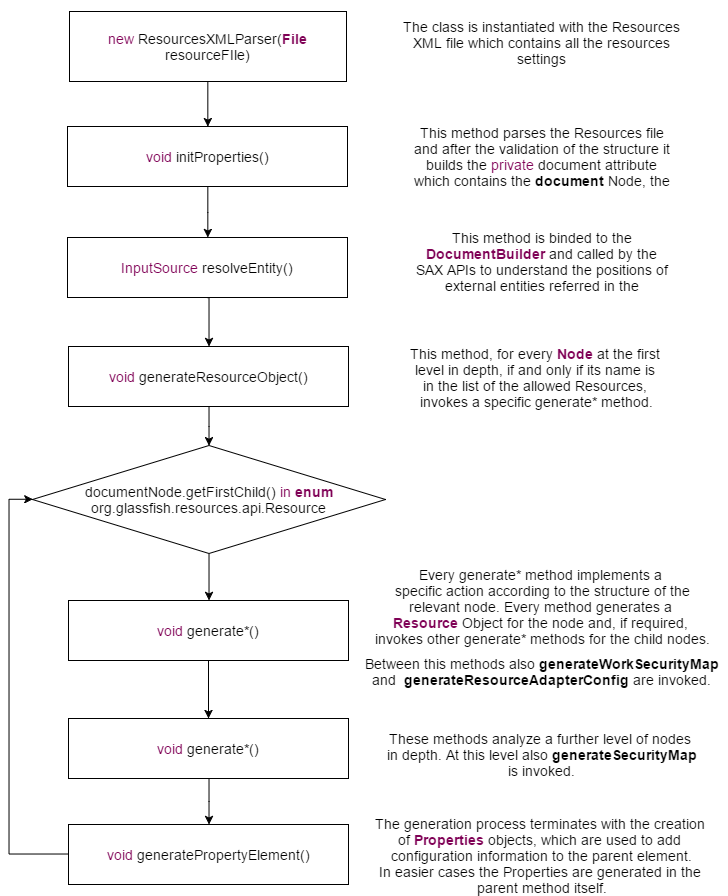
\includegraphics[width=1\columnwidth]{FlowChart}
        \caption{High level flow chart of class execution}
        \label{fig:flowchart}
\end{figure}

\subsection{Method: resolveEntity}
In the resolveEntity method, firstly, the DTD version is identified, comparing the publicId and systemId parameters with a preset list of names, and then if the DTD file is present, it is loaded as an InputStream otherwise an Exception is thrown.

\subsection{Method: generateWorkSecurityMap}
The method generateWorkSecurityMap is called by generateResourceObjects if the name of the node in exam is CONNECTOR\_WORK\_SECURITY\_MAP. It creates a Resource object and sets two attributes of the object with the value of the relevant attributes of the node. Then for all the children nodes that are \\WORK\_SECURITY\_MAP\_GROUP\_MAP or \\WORK\_SECURITY\_MAP\_PRINCIPAL\_MAP it add other attributes to the resource with the value of the relevant nodes.\\
Finally the resource is added to the collection of resources and to the map.

\subsection{Method: generateSecurityMap}
The method generateSecurityMap is called by generateConnectorConnectionPoolResource if the name of the node in exam is SECURITY\_MAP. A resource for the node is created and few basic attributes of the resource are added. Then the children nodes are extracted and if their names are SECURITY\_MAP\_PRINCIPAL or SECURITY\_MAP\_USER\_GROUP the first child is extracted and the value inserted in a String array that are then inserted as attributes of the Resource. If the child node is, instead, a SECURITY\_MAP\_BACKEND\_PRINCIPAL, the values of its attributes USER\_NAME and PASSWORD are directly added as attributes of the resource. The resource is finally added to the collection of resources and to the map.

\subsection{Method: generateResourceAdapterConfig}
The method generateResourceAdapterConfig is called by generateResourceObjects if the name of the node in exam is RESOURCE\_ADAPTER\_CONFIG. As before, a Resource element is created and the attributes of the nodes are added to the resource. The resource is then added to the the collection of resources and to the map.